\documentclass[a4paper]{article}

\def\npart {II}
\def\nterm {Michaelmas}
\def\nyear {2015}
\def\nlecturer {H. Wilton}
\def\ncourse {Algebraic Topology}
\def\nlectures {MWF.9}
\def\nnotready {}

% Imports
\ifx \nextra \undefined
  \usepackage[pdftex,
    hidelinks,
    pdfauthor={Dexter Chua},
    pdfsubject={Cambridge Maths Notes: Part \npart\ - \ncourse},
    pdftitle={Part \npart\ - \ncourse},
  pdfkeywords={Cambridge Mathematics Maths Math \npart\ \nterm\ \nyear\ \ncourse}]{hyperref}
  \title{Part \npart\ - \ncourse}
\else
  \usepackage[pdftex,
    hidelinks,
    pdfauthor={Dexter Chua},
    pdfsubject={Cambridge Maths Notes: Part \npart\ - \ncourse\ (\nextra)},
    pdftitle={Part \npart\ - \ncourse\ (\nextra)},
  pdfkeywords={Cambridge Mathematics Maths Math \npart\ \nterm\ \nyear\ \ncourse\ \nextra}]{hyperref}

  \title{Part \npart\ - \ncourse \\ {\Large \nextra}}
\fi

\author{Lectured by \nlecturer \\\small Notes taken by Dexter Chua}
\date{\nterm\ \nyear}

\usepackage{alltt}
\usepackage{amsfonts}
\usepackage{amsmath}
\usepackage{amssymb}
\usepackage{amsthm}
\usepackage{booktabs}
\usepackage{caption}
\usepackage{enumitem}
\usepackage{fancyhdr}
\usepackage{graphicx}
\usepackage{mathtools}
\usepackage{microtype}
\usepackage{multirow}
\usepackage{pdflscape}
\usepackage{pgfplots}
\usepackage{siunitx}
\usepackage{tabularx}
\usepackage{tikz}
\usepackage{tkz-euclide}
\usepackage[normalem]{ulem}
\usepackage[all]{xy}

\pgfplotsset{compat=1.12}

\pagestyle{fancyplain}
\lhead{\emph{\nouppercase{\leftmark}}}
\ifx \nextra \undefined
  \rhead{
    \ifnum\thepage=1
    \else
      \npart\ \ncourse
    \fi}
\else
  \rhead{
    \ifnum\thepage=1
    \else
      \npart\ \ncourse\ (\nextra)
    \fi}
\fi
\usetikzlibrary{arrows}
\usetikzlibrary{decorations.markings}
\usetikzlibrary{decorations.pathmorphing}
\usetikzlibrary{positioning}
\usetikzlibrary{fadings}
\usetikzlibrary{intersections}
\usetikzlibrary{cd}

\newcommand*{\Cdot}{\raisebox{-0.25ex}{\scalebox{1.5}{$\cdot$}}}
\newcommand {\pd}[2][ ]{
  \ifx #1 { }
    \frac{\partial}{\partial #2}
  \else
    \frac{\partial^{#1}}{\partial #2^{#1}}
  \fi
}

% Theorems
\theoremstyle{definition}
\newtheorem*{aim}{Aim}
\newtheorem*{axiom}{Axiom}
\newtheorem*{claim}{Claim}
\newtheorem*{cor}{Corollary}
\newtheorem*{defi}{Definition}
\newtheorem*{eg}{Example}
\newtheorem*{fact}{Fact}
\newtheorem*{law}{Law}
\newtheorem*{lemma}{Lemma}
\newtheorem*{notation}{Notation}
\newtheorem*{prop}{Proposition}
\newtheorem*{thm}{Theorem}

\renewcommand{\labelitemi}{--}
\renewcommand{\labelitemii}{$\circ$}
\renewcommand{\labelenumi}{(\roman{*})}

\let\stdsection\section
\renewcommand\section{\newpage\stdsection}

% Strike through
\def\st{\bgroup \ULdepth=-.55ex \ULset}

% Maths symbols
\newcommand{\bra}{\langle}
\newcommand{\ket}{\rangle}

\newcommand{\N}{\mathbb{N}}
\newcommand{\Z}{\mathbb{Z}}
\newcommand{\Q}{\mathbb{Q}}
\renewcommand{\H}{\mathbb{H}}
\newcommand{\R}{\mathbb{R}}
\newcommand{\C}{\mathbb{C}}
\newcommand{\Prob}{\mathbb{P}}
\renewcommand{\P}{\mathbb{P}}
\newcommand{\E}{\mathbb{E}}
\newcommand{\F}{\mathbb{F}}
\newcommand{\cU}{\mathcal{U}}
\newcommand{\RP}{\mathbb{RP}}
\newcommand{\CP}{\mathbb{CP}}

\newcommand{\ph}{\,\cdot\,}

\DeclareMathOperator{\sech}{sech}
\DeclareMathOperator{\cosech}{cosech}
\DeclareMathOperator{\cosec}{cosec}

\DeclareMathOperator{\covol}{covol}
\DeclareMathOperator{\vol}{vol}

\let\Im\relax
\let\Re\relax
\DeclareMathOperator{\Im}{Im}
\DeclareMathOperator{\Re}{Re}
\DeclareMathOperator{\im}{im}
\DeclareMathOperator{\image}{image}
\DeclareMathOperator{\Ann}{Ann}

\DeclareMathOperator*{\res}{res}
\DeclareMathOperator{\Res}{Res}
\DeclareMathOperator{\Ind}{Ind}

\DeclareMathOperator{\tr}{tr}
\DeclareMathOperator{\diag}{diag}
\DeclareMathOperator{\rank}{rank}
\DeclareMathOperator{\card}{card}
\DeclareMathOperator{\spn}{span}
\DeclareMathOperator{\adj}{adj}

\DeclareMathOperator{\erf}{erf}
\DeclareMathOperator{\erfc}{erfc}

\DeclareMathOperator{\ord}{ord}
\DeclareMathOperator{\Sym}{Sym}

\DeclareMathOperator{\sgn}{sgn}
\DeclareMathOperator{\orb}{orb}
\DeclareMathOperator{\stab}{stab}
\DeclareMathOperator{\ccl}{ccl}

\DeclareMathOperator{\lcm}{lcm}
\DeclareMathOperator{\hcf}{hcf}

\DeclareMathOperator{\Int}{Int}
\DeclareMathOperator{\id}{id}

\DeclareMathOperator{\betaD}{beta}
\DeclareMathOperator{\gammaD}{gamma}
\DeclareMathOperator{\Poisson}{Poisson}
\DeclareMathOperator{\binomial}{binomial}
\DeclareMathOperator{\multinomial}{multinomial}
\DeclareMathOperator{\Bernoulli}{Bernoulli}
\DeclareMathOperator{\like}{like}

\DeclareMathOperator{\var}{var}
\DeclareMathOperator{\cov}{cov}
\DeclareMathOperator{\bias}{bias}
\DeclareMathOperator{\mse}{mse}
\DeclareMathOperator{\corr}{corr}

\DeclareMathOperator{\otp}{otp}
\DeclareMathOperator{\dom}{dom}

\DeclareMathOperator{\Root}{Root}
\DeclareMathOperator{\supp}{supp}
\DeclareMathOperator{\rel}{rel}
\DeclareMathOperator{\Hom}{Hom}
\DeclareMathOperator{\Aut}{Aut}
\DeclareMathOperator{\Gal}{Gal}
\DeclareMathOperator{\Mat}{Mat}
\DeclareMathOperator{\End}{End}
\DeclareMathOperator{\Char}{char}
\DeclareMathOperator{\ev}{ev}
\DeclareMathOperator{\St}{St}
\DeclareMathOperator{\Lk}{Lk}
\DeclareMathOperator{\disc}{disc}
\DeclareMathOperator{\Isom}{Isom}
\DeclareMathOperator{\length}{length}
\DeclareMathOperator{\energy}{energy}
\DeclareMathOperator{\area}{area}
\DeclareMathOperator{\Syl}{Syl}
\DeclareMathOperator{\cl}{cl}
\DeclareMathOperator{\fix}{fix}

\newcommand{\GL}{\mathrm{GL}}
\newcommand{\SL}{\mathrm{SL}}
\newcommand{\PGL}{\mathrm{PGL}}
\newcommand{\PSL}{\mathrm{PSL}}
\newcommand{\PSU}{\mathrm{PSU}}
\newcommand{\Or}{\mathrm{O}}
\newcommand{\SO}{\mathrm{SO}}
\newcommand{\U}{\mathrm{U}}
\newcommand{\SU}{\mathrm{SU}}

\renewcommand{\d}{\mathrm{d}}
\newcommand{\D}{\mathrm{D}}

\tikzset{->/.style = {decoration={markings,
                                  mark=at position 1 with {\arrow[scale=2]{latex'}}},
                      postaction={decorate}}}
\tikzset{<-/.style = {decoration={markings,
                                  mark=at position 0 with {\arrowreversed[scale=2]{latex'}}},
                      postaction={decorate}}}
\tikzset{<->/.style = {decoration={markings,
                                   mark=at position 0 with {\arrowreversed[scale=2]{latex'}},
                                   mark=at position 1 with {\arrow[scale=2]{latex'}}},
                       postaction={decorate}}}
\tikzset{->-/.style = {decoration={markings,
                                   mark=at position #1 with {\arrow[scale=2]{latex'}}},
                       postaction={decorate}}}
\tikzset{-<-/.style = {decoration={markings,
                                   mark=at position #1 with {\arrowreversed[scale=2]{latex'}}},
                       postaction={decorate}}}

\tikzset{circ/.style = {fill, circle, inner sep = 0, minimum size = 3}}
\tikzset{mstate/.style={circle, draw, blue, text=black, minimum width=0.7cm}}

\definecolor{mblue}{rgb}{0.2, 0.3, 0.8}
\definecolor{morange}{rgb}{1, 0.5, 0}
\definecolor{mgreen}{rgb}{0.1, 0.4, 0.2}
\definecolor{mred}{rgb}{0.5, 0, 0}

\def\drawcirculararc(#1,#2)(#3,#4)(#5,#6){%
    \pgfmathsetmacro\cA{(#1*#1+#2*#2-#3*#3-#4*#4)/2}%
    \pgfmathsetmacro\cB{(#1*#1+#2*#2-#5*#5-#6*#6)/2}%
    \pgfmathsetmacro\cy{(\cB*(#1-#3)-\cA*(#1-#5))/%
                        ((#2-#6)*(#1-#3)-(#2-#4)*(#1-#5))}%
    \pgfmathsetmacro\cx{(\cA-\cy*(#2-#4))/(#1-#3)}%
    \pgfmathsetmacro\cr{sqrt((#1-\cx)*(#1-\cx)+(#2-\cy)*(#2-\cy))}%
    \pgfmathsetmacro\cA{atan2(#2-\cy,#1-\cx)}%
    \pgfmathsetmacro\cB{atan2(#6-\cy,#5-\cx)}%
    \pgfmathparse{\cB<\cA}%
    \ifnum\pgfmathresult=1
        \pgfmathsetmacro\cB{\cB+360}%
    \fi
    \draw (#1,#2) arc (\cA:\cB:\cr);%
}
\newcommand\getCoord[3]{\newdimen{#1}\newdimen{#2}\pgfextractx{#1}{\pgfpointanchor{#3}{center}}\pgfextracty{#2}{\pgfpointanchor{#3}{center}}}

\def\Xint#1{\mathchoice
   {\XXint\displaystyle\textstyle{#1}}%
   {\XXint\textstyle\scriptstyle{#1}}%
   {\XXint\scriptstyle\scriptscriptstyle{#1}}%
   {\XXint\scriptscriptstyle\scriptscriptstyle{#1}}%
   \!\int}
\def\XXint#1#2#3{{\setbox0=\hbox{$#1{#2#3}{\int}$}
     \vcenter{\hbox{$#2#3$}}\kern-.5\wd0}}
\def\ddashint{\Xint=}
\def\dashint{\Xint-}


\begin{document}
\maketitle
{\small
\noindent\textbf{The fundamental group}\\
Homotopy of continuous functions and homotopy equivalence between topological spaces. The fundamental group of a space, homomorphisms induced by maps of spaces, change of base point, invariance under homotopy equivalence.\hspace*{\fill} [3]

\vspace{10pt}
\noindent\textbf{Covering spaces}\\
Covering spaces and covering maps. Path-lifting and homotopy-lifting properties, and their application to the calculation of fundamental groups. The fundamental group of the circle; topological proof of the fundamental theorem of algebra. *Construction of the universal covering of a path-connected, locally simply connected space*. The correspondence between connected coverings of $X$ and conjugacy classes of subgroups of the fundamental group of $X$.\hspace*{\fill} [5]

\vspace{10pt}
\noindent\textbf{The Seifert-Van Kampen theorem}\\
Free groups, generators and relations for groups, free products with amalgamation. Statement *and proof* of the Seifert-Van Kampen theorem. Applications to the calculation of fundamental groups.\hspace*{\fill} [4]

\vspace{10pt}
\noindent\textbf{Simplicial complexes}\\
Finite simplicial complexes and subdivisions; the simplicial approximation theorem.\hspace*{\fill} [3]

\vspace{10pt}
\noindent\textbf{Homology}\\
Simplicial homology, the homology groups of a simplex and its boundary. Functorial properties for simplicial maps. *Proof of functoriality for continuous maps, and of homotopy invariance*.\hspace*{\fill} [4]

\vspace{10pt}
\noindent\textbf{Homology calculations}\\
The homology groups of $S^n$, applications including Brouwer's fixed-point theorem. The Mayer-Vietoris theorem. *Sketch of the classification of closed combinatorical surfaces*; determination of their homology groups. Rational homology groups; the Euler-Poincar\'e characteristic and the Lefschetz fixed-point theorem.\hspace*{\fill} [5]}

\tableofcontents

\setcounter{section}{-1}
\section{Introduction}
In topology, a typical problem is that we have two spaces $X$ and $Y$, and we want to know if $X\cong Y$, ie. if $X$ and $Y$ are homeomorphic. If they are homeomorphic, we can easily show this by writing down a homeomorphism. But what if they are not? How can we prove that two spaces are not homeomorphic?

For example, are $\R^m$ and $\R^n$ homeomorphic (for $m\not= n$)? Intuitively, they should not be, since they have different dimensions, and in fact they are. But how can we actually prove this?

The idea of algebraic topology is to translate these non-existence problems in topology to non-existence problems in algebra. It turns out we are much better at algebra than topology. It is \emph{much} easier to show that two groups are not isomorphic.

While the statement that $\R^m \not\cong \R^n$ for $n \not= m$ is intuitively obvious, algebraic topology can be used to prove some less obvious results.

Let $D^n$ be the $n$ dimensional unit disk, and $S^{n - 1}$ be the $n-1$ dimensional unit sphere. We will be able to show that there is no continuous map $F: D^n \to S^{n - 1}$ such that the composition
\[
  \begin{tikzcd}
    S^{n - 1} \ar[r, hook] & D^n \ar[r, "F"] & S^{n - 1}
  \end{tikzcd}
\]
is the identity, where the first arrow is the inclusion map. Alternatively, this says that we cannot continuously map the disk onto the boundary sphere such that the boundary sphere is fixed by the map.

Using algebraic topology, we can translate this statement into an algebraic statement: there is no homomorphism $F: \{0\} \to \Z$ such that
\[
  \begin{tikzcd}
    \Z \ar[r, hook] & \{0\} \ar[r, "F"] & \Z
  \end{tikzcd}
\]
is the identity. This is something we can prove in 5 seconds.

By translating a non-existence problem of a continuous map to a non-existence problem of a homomorphism, we have made our life much easier.

In algebraic topology, we will be developing a lot of machinery to do this sort of translation. However, this machinery is not easy. It will take some hard work, and will be rather tedious and boring at the beginning. So keep in mind that the point of all that hard work is to prove all these interesting theorems.

In case you are completely uninterested in topology, and don't care if $\R^m$ and $\R^n$ are homeomorphic, further applications of algebraic topology include \emph{solving equations}. For example, we will be able to prove the fundamental theorem of algebra, as well as Brouwer's fixed point theorem (which says that every continuous function from $D^2 \to D^2$ has a fixed point). If you are not interested in these as well, you may as well drop this course.

\section{Definitions}
\subsection{Some recollections and conventions}
We will start with some preliminary definitions and conventions.

\begin{defi}[Map]
  In this course, the word \emph{map} will always refer to continuous maps. We are doing topology, and never care about non-continuous functions.
\end{defi}

We are going to build a lot of continuous maps in algebraic topology. To do so, we will often need to glue maps together. The \emph{glueing lemma} tells us that this works.
\begin{lemma}[Glueing lemma]
  If $f: X\to Y$ is a function of topological spaces, $X = C\cup K$, $C$ and $K$ are both closed, then $f$ is continuous if and only if the restrictions $f|_C$ and $f|_K$are continuous.
\end{lemma}
The proof is easy from the definition of continuous maps.

\subsection{Cell complexes}
In general, we can construct some really horrible topological spaces. Even if we require them to be compact, Hausdorff etc, we can often still produce really ugly topological spaces. In algebraic topology, we will often restrict our attention to some nice topological spaces, known as \emph{cell complexes}.

To build cell complexes, we are not just glueing maps, but spaces.

\begin{defi}[Cell attachment]
  Fora a space $X$, and a map $f: S^{n - 1}\to X$, the space obtained by \emph{attaching an $n$-cell} to $X$ along $f$ is
  \[
    X\cup_{f}D^n = (X\sqcup D^N)/{\sim},
  \]
  where the equivalence relation $\sim$ is the equivalence relation generated by $x\sim f(x)$ for all $x\in S^{n - 1}\subseteq D^n$.

  Intuitively, a map $f: S^{n - 1}\to X$ is just picks out a subset $X$ that looks like the sphere. So we are just sticking a disk onto $X$ by attaching the boundary of the disk onto a sphere within $X$.
  \begin{center}
    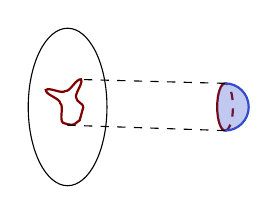
\begin{tikzpicture}
      \draw ellipse (0.5 and 1);

      \draw [thick, mred, decorate, decoration={snake}] circle [radius=0.2];

      \draw [thick, mred] (2, 0.3) arc (90:270:0.1 and 0.3);
      \draw [dashed, thick, mred] (2, -0.3) arc (270:450:0.1 and 0.3);

      \fill [mblue, opacity=0.3] (2, 0.3) arc (90:270:0.1 and 0.3) arc (270:450:0.3);
      \draw [thick, mblue] (2, -0.3) arc (270:450:0.3);

      \draw [dashed] (2, 0.3) -- (0.12, 0.35);
      \draw [dashed] (2, -0.3) -- (-0.05, -0.23);
    \end{tikzpicture}
  \end{center}
\end{defi}

\begin{defi}[Cell complex]
  A (finite) \emph{cell complex} is a space $X$ obtained by
  \begin{enumerate}
    \item Start with a discrete finite set $X^{(0)}$.
      \begin{center}
        \begin{tikzpicture}
          \node [circ] at (0, 0) {};
          \node [circ] at (-1, -1.2) {};
          \node [circ] at (1, -1) {};
          \node [circ] at (0.3, -2) {};
        \end{tikzpicture}
      \end{center}
    \item Given $X^{n - 1}$, for $X^n$ by taking a finite set of maps $\{f_\alpha: S^{n - 1} \to X^{(n - 1)}\}$  by attaching $n$-cells along the $f_\alpha$:
      \[
        X^{(n)} = \left(X^{(n - 1)}\sqcup \bigsqcup_\alpha D_{\alpha}^N\right)/\{x\sim f_\alpha(x)\}.
      \]
      For example, given the $X^{(0)}$ above, we can attach some loops and lines to obtain the following $X^{(1)}$
      \begin{center}
        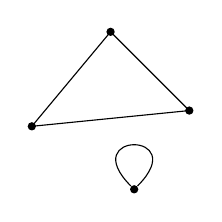
\begin{tikzpicture}
          \node [circ] at (0, 0) {};
          \node [circ] at (-1, -1.2) {};
          \node [circ] at (1, -1) {};
          \node [circ] (3) at (0.3, -2) {};

          \draw (0, 0) -- (-1, -1.2) -- (1, -1) -- (0, 0);
          \draw (3) edge [loop, looseness=30] (3);
        \end{tikzpicture}
      \end{center}
      We can add surfaces to obtain the following $X^{(2)}$
      \begin{center}
        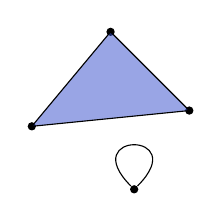
\begin{tikzpicture}
          \node [circ] at (0, 0) {};
          \node [circ] at (-1, -1.2) {};
          \node [circ] at (1, -1) {};
          \node [circ] (3) at (0.3, -2) {};

          \draw [fill = mblue, fill opacity=0.5] (0, 0) -- (-1, -1.2) -- (1, -1) -- (0, 0);
          \draw (3) edge [loop, looseness=30] (3);
        \end{tikzpicture}
      \end{center}
    \item Stop at some $X = X^{(k)}$. The minimum such $k$ is the \emph{dimension} of $X$.
  \end{enumerate}
  To define non-finite cell complexes, we just have to remove the words ``finite'' in the definition and remove the final condition.
\end{defi}

\begin{eg}
  The following is \emph{not} a cell complex: we take $\R^2$, and add a circle with radius $\frac{1}{2}$ and center $(0, \frac{1}{2})$. Then we add another circle with radius $\frac{1}{4}$ and center $(0, \frac{1}{4})$, then a circle with radius $\frac{1}{8}$ and center $(0, \frac{1}{8})$ etc. We obtain something like
  \begin{center}
    \begin{tikzpicture}[scale=2]
      \draw (0, 0.5) circle [radius=0.5];
      \draw (0, 0.25) circle [radius=0.25];
      \draw (0, 0.125) circle [radius = 0.125];
      \draw (0, 0.0625) circle [radius = 0.0625];
      \draw [gray] (-2, 0) -- (2, 0);

      \node [circ, mblue] at (0, 1) {};
      \node [circ, mblue] at (0, 0.5) {};
      \node [circ, mblue] at (0, 0.25) {};
      \node [circ, mblue] at (0, 0.125) {};
    \end{tikzpicture}
  \end{center}
  This is known as the \emph{Hawaiian Earring}.

  Why is this not an (infinite) cell complex? We did obtain it by attaching 1-cells to the single point $(0, 0)$. However, when attaching cells to a cell complex, the cells should not be ``close'' to each other. They are completely separated from each other apart from touching at the origin. However, here the circles clump together at the origin.

  In particular, if we take the following sequence $(0, 1), (0, \frac{1}{2}), (0, \frac{1}{4}), \cdots$, it converges to $(0, 0)$. If this were a cell complex, then this shouldn't happen because the cells are unrelated, and picking a point from each cell should not produce a convergent sequence (if you are not convinced, if we actually did produce by attaching cells, then note that during the attaching process, we needn't have attached them this way. We could have made it such that the $n$th cell has radius $n$. Then clearly picking the topmost point of each cell will not produce a convergent sequence).

  We will see that the Hawaiian Earring will be a counterexample to a lot of our theorems here.
\end{eg}

\section{Homotopy and the fundamental group}
This will be our first trick to translate topological spaces into groups.

\setcounter{subsection}{-1}
\subsection{Motivation}
Recall that we wanted to prove that $\R^n \not\cong \R^m$ for $n\not= m$. Let's first do the simple case, where $m = 1, n = 2$. We want to show that $\R\not\cong \R^2$.

This is not hard. We know that $\R$ is a line, while $\R^2$ is a plane. Let's try to remove a point from each of them.  If we remove a point from $\R$, the space stops being path connected. However, removing a point does not have this effect on $\R^2$. Since being path connected is a topological property, we have now showed that $\R$ and $\R^2$ are not homeomorphic.

Unfortunately, this does not extend very far. We cannot use this to show that $\R^2$ and $\R^3$ are not homeomorphic. What else can we do?

Notice that when we remove a point from $\R^2$, sure it is still connected, but something has changed.

Consider a circle containing the origin in $\R^2 \setminus \{0\}$. If the origin were there, we can keep shrinking the circle down until it becomes a point. However, we cannot do this if the origin is missing.
\begin{center}
  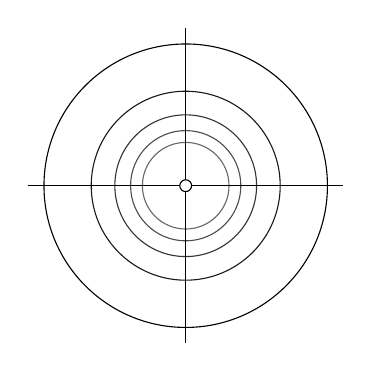
\begin{tikzpicture}
    \draw (-2, 0) -- (2, 0);
    \draw (0, -2) -- (0, 2);

    \draw [fill=white] circle [radius=0.075];
    \draw circle [radius=1.8];
    \draw [opacity=0.9] circle [radius=1.2];
    \draw [opacity=0.8] circle [radius=0.9];
    \draw [opacity=0.7] circle [radius=0.7];
    \draw [opacity=0.6] circle [radius=0.55];
  \end{tikzpicture}
\end{center}
The strategy now is to exploit the fact that $\R^2 \setminus \{0\}$ has circles which cannot be deformed to points.

\subsection{Homotopy}
We have just talked about the notion of ``deforming'' circles to a point. We can think of a circle in $X$ as a map $S^1 \to X$, and we want to ``deform'' this map to a point. This process of deformation is known as \emph{homotopy}. Here we are going to use the interval $[0, 1]\subseteq \R $ a lot, and we will just call it $I$.
\begin{notation}
  \[
    I = [0, 1]\subseteq \R.
  \]
\end{notation}

\begin{defi}[Homotopy]
  Let $f, g: X\to Y$ be maps. A \emph{homotopy} from $f$ to $g$ is a map
  \[
    H: X\times I \to Y
  \]
  such that
  \[
    H(x, 0) = f(x),\quad H(x, 1) = g(x).
  \]
  We think of the interval $I$ as time. For each time $t$, $H(\cdot, t)$ defines a map $X\to Y$. So we want to start from $f$, move with time, and eventually reach $g$.

  If such an $H$ exists, we say $f$ is \emph{homotopic} to $g$, and write $f\simeq g$. If we want to make it explicit that the homotopy is $H$, we write $f \simeq_H g$.
\end{defi}
As mentioned at the beginning, by calling $H$ a map, we are requiring it to be continuous.

Sometimes, we don't want a general homotopy. We might want to make sure that when we are deforming from a path $f$ to $g$, the end points of the path don't move. In general, we have
\begin{defi}[Homotopy $\rel$ A]
  $f$ is \emph{homotopic to} $g$ \emph{rel} $A$, written $f\simeq g\rel A$, if for all $a \in A\subseteq X$, we have
  \[
    H(a, t) = f(a) = g(a).
  \]
\end{defi}
This notion will find itself useful later, but we don't have to pay too much attention to this yet.

Our notation suggests that homotopy is an equivalence relation. Indeed, we have
\begin{prop}
  For spaces $X, Y$, and $A\subseteq X$, the ``homotopic $\rel A$'' relation is an equivalence relation. In particular, when $A = \emptyset$, homotopy is an equivalence relation.
\end{prop}

\begin{proof}\leavevmode
  \begin{enumerate}
    \item Reflexivity: $f \simeq f$ since $H(x, t) = f(x)$ is a homotopy.
    \item Symmetry: is $H(x, t)$ is a homotopy from $f$ to $g$, then $H(x, 1 - t)$ is a homotopy from $g$ to $h$.
    \item Transitivity: Suppose $f, g, h: X\to Y$ and $f\simeq_H g\rel A$, $g\simeq_{H'} h \rel A$. We want to show that $f\simeq h \rel A$. The idea is to ``glue'' the two maps together.

      We know how to continuously deform $f$ to $g$, and from $g$ to $h$. So we just do these one after another.
      We define $H'': X\times I \to Y$ by
      \[
        H(x, t) =
        \begin{cases}
          H(x, 2t) & 0 \leq t \leq \frac{1}{2}\\
          H'(x, 2t - 1) & \frac{1}{2} \leq t \leq 1
        \end{cases}
      \]
      This is well-defined since $H(x, 1) = g(x) = H'(x, 0)$. This is also continuous by the gluing lemma. It is easy to check that $H''$ is a homotopy $\rel A$.
  \end{enumerate}
\end{proof}

We now have a notion of equivalence of maps - two maps are equivalent if they are homotopic. We can extend the notion of homotopy to spaces as well.

Recall that when we defined homeomorphism, we required that there is some $f, g$ such that $f\circ g = \id$, $g\circ f = \id$. Here, we replace equality by homotopy.
\begin{defi}[Homotopy equivalence]
  A map $f: X\to Y$ is a \emph{homotopy equivalence} if there exists a $g: Y\to X$ such that $f\circ g \simeq \id_Y$ and $g\circ f \simeq \id_X$. We call $g$ a \emph{homotopy inverse} for $f$.

  If a homotopy equivalence $f: X\to Y$ exists, we say that $X$ and $Y$ are homotopy equivalent and write $X\simeq Y$.
\end{defi}
We are soon going to prove that this is indeed an equivalence relation on spaces, but we first look at some examples of homotopy equivalent spaces. Clearly, homeomorphic spaces are homotopy equivalent. However, we will see that we can do much more ``violent'' things to a space and still be homotopy equivalent.
\begin{eg}
  Let $X = S^1$, $Y = \R^2 \setminus \{0\}$. We have a natural inclusion map $i: X\hookrightarrow Y$. To obtain a map $Y \to X$, we can project each point onto the circle.
  \begin{center}
    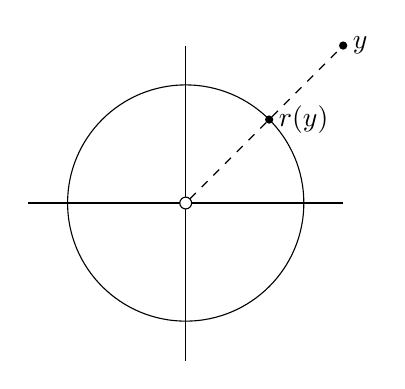
\begin{tikzpicture}
      \draw (-2, 0) -- (2, 0);
      \draw (0, -2) -- (0, 2);

      \draw [fill=white] circle [radius=0.075];
      \draw circle [radius=1.5];

      \node [circ] at (1.06, 1.06) {};
      \node [circ] at (2, 2) {};
      \node at (1.06, 1.06) [right] {$r(y)$};
      \node at (2, 2) [right] {$y$};
      \draw [dashed] (0.053, 0.053) -- (2, 2);
    \end{tikzpicture}
  \end{center}
  In particular, we define $r: Y\to X$ by
  \[
    r(y) = \frac{y}{\|y\|}.
  \]
  We immediately have $r\circ i = \id_X$. We will now see that $i\circ r \simeq \id_Y$. The composition $i\circ r$ first projects each object into $S^1$, and then includes it back into $\R^2 \setminus \{0\}$. So this is just the projection map. We can define a homotopy $H: Y\times I \to Y$ by
  \[
    H(y, t) = \frac{y}{t + (1 - t)\|y\|}.
  \]
  This is continuous, and $H(\cdot, 0) = i\circ r$, $H(\cdot, 1) = \id_Y$.
\end{eg}
As we have said, homotopy equivalence can do really ``violent'' things to a space. We started with a 2-dimensional $\R^2\setminus \{0\}$ space, and squashed it into a one-dimensional sphere.

Hence we see that homotopy doesn't \emph{care} about dimensions. This seems to be a rather fundamental thing in geometry, and we are discarding it. So what is left? What does homotopy preserve?

While $S^1$ and $\R^2 \setminus \{0\}$ seem rather different, they have something in common - they both have a ``hole''. We will later see that this is what homotopy preserves.

\begin{eg}
  Let $Y = \R^n$, $X = \{0\} = *$. Let $X\hookrightarrow Y$ be the inclusion map, and $r: Y\to X$ be the unique map that sends everything to $\{0\}$. Again, we have $r\circ i = \id_X$. We can also obtain a homotopy from $i \circ r$ to $\id_Y$ by
  \[
    H(y, t) = ty.
  \]
\end{eg}
Again, from the point of view of homotopy theory, $\R^n$ is just the same as a point! You might think that this is something crazy to do - we have just given up a lot of structure of topological spaces. However, this turns out to be a really useful notion.

In general things homotopic to a single point are known as \emph{contractible spaces}.
\begin{notation}
  $*$ denotes the one-point space $\{0\}$.
\end{notation}

\begin{defi}[Contractible space]
  If $X\simeq *$, then $X$ is \emph{contractible}.
\end{defi}

We now show that homotopy of spaces is an equivalence relation. To do this, we first need a lemma.
\begin{lemma}
  Consider the spaces and arrows
  \[
    \begin{tikzcd}
      X \ar[r, bend left, "f_0"] \ar[r, bend right, "f_1"'] & Y \ar[r, bend left, "g_0"] \ar[r, bend right, "g_1"'] & Z
    \end{tikzcd}
  \]
  If $f_0\simeq_H f_1$ and $g_0\simeq_{H'} g_1$, then $g_0\circ f_0 \simeq g_1 \circ f_1$.
\end{lemma}

\begin{proof}
  We will show that $g_0 \circ f_0 \simeq g_0 \circ f_1 \simeq g_1 \circ f_1$. Then we are done since homotopy between maps is an equivalence relation. So we need to write down two homotopies.

  \begin{enumerate}
    \item Consider the following composition:
      \[
        \begin{tikzcd}
          X\times I \ar[r, "H"] & Y \ar[r, "g_0"] & Z
        \end{tikzcd}
      \]
      It is easy to check that this is the first homotopy we need to show $g_0\circ f_0 = g_0 \circ f_1$.
    \item The following composition is a homotopy from $g_0 \circ f_1$ to $g_1 \circ f_1$:
      \[
        \begin{tikzcd}
          X\times I \ar[r, "f_1\times \id_I"] & Y\times I \ar[r, "H'"] & Z
        \end{tikzcd}
      \]
  \end{enumerate}
\end{proof}

\begin{prop}
  Homotopy on spaces is a equivalence relation.
\end{prop}

\begin{proof}(sketch)
  Symmetry and reflexivity are trivial, and applying the previous lemma several times can show transitivity.
\end{proof}

\begin{defi}[Retraction]
  Let $A\subseteq X$ be a subspace. A \emph{retraction} $r: X\to A$ is a map such that $r\circ i = \id_A$, where $i: A\hookrightarrow X$ is the inclusion.
\end{defi}
This map sends everything in $X$ to $A$ without mmoving things in $A$. Roughly speaking, if such a retraction exists, then $A$ is no more complicated than $X$.

\begin{defi}{Deformation retraction}
  The retraction $r$ is a \emph{deformation retraction} if $i\circ r \simeq \id_X$. Some authors requires that this homotopy is a homotopy rel $A$.
\end{defi}
Roughly, this says that $A$ is as complicated as $X$.

\begin{eg}
Take $X$ any space, and $A = \{x\}\subseteq X$. Then the constant map $r: X\to A$ is a retraction. If $X$ is contractible, then this is a deformation retract.
\end{eg}

\subsection{Paths}
\begin{defi}[Path]
  A \emph{path} in a space $X$ is a map $\gamma: I\to X$. If $\gamma(0) = x_0$ and $\gamma(1) = x_1$, we say $\gamma$ is a path from $x_0$ to $x_1$, and write $\gamma: x_0 \rightsquigarrow x_1$.

  If $\gamma(0) = \gamma(1)$, then $\gamma$ is called a \emph{loop} (based at $x_0$).
  \begin{center}
    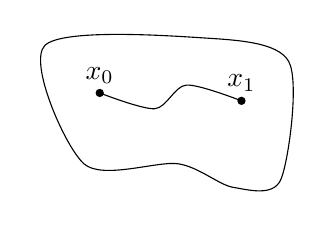
\begin{tikzpicture}
      \draw plot [smooth cycle] coordinates {(-1.2, -0.7) (0, -0.7) (0.7, -1) (1.3, -0.9) (1.4, 0.6) (0.3, 0.9) (-1.7, 0.8)};

      \node [circ] at (-1, 0.2) {};
      \node [above] at (-1, 0.2) {$x_0$};
      \node [circ] at (0.8, 0.1) {};
      \node [above] at (0.8, 0.1) {$x_1$};
      \draw plot [smooth] coordinates {(-1, 0.2) (-0.3, 0) (0.1, 0.3) (0.8, 0.1)};
    \end{tikzpicture}
  \end{center}
\end{defi}
Note that this map does not have to be injective. It can be self intersecting or do all sorts of weird stuff.

Recall that the basic idea of algebraic topology is to assign to each space $X$ an (algebraic) object, which is (hopefully) easier to deal with. In homotopy theory, we do so using the idea of paths.

To do so, we need to be able to perform operations on paths.
\begin{defi}[Concatenation of paths]
  If we have two paths $\gamma_1$ from $x_0$ to $x_1$; and $\gamma_2$ from $x_1$ to $x_2$, we define the \emph{concatenation to be}
  \[
    (\gamma_1\cdot \gamma_2)(t) =
    \begin{cases}
      \gamma(2t) & 0 \leq t \leq \frac{1}{2}\\
      \gamma(2t - 1) & \frac{1}{2} \leq t \leq 1.
    \end{cases}
  \]
  This is continuous by the gluing lemma.
\end{defi}
Note that we concatenate left to right, but function composition goes from right to left.
\begin{center}
  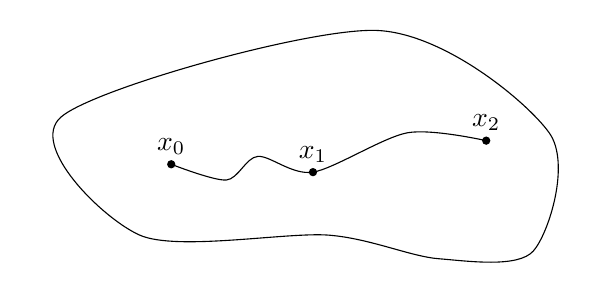
\begin{tikzpicture}
    \draw plot [smooth cycle] coordinates {(-2.4, -0.7) (0, -0.7) (1.4, -1) (2.6, -0.9) (2.8, 0.6) (0.6, 1.9) (-3.4, 0.8)};

    \node [circ] at (-2, 0.2) {};
    \node [above] at (-2, 0.2) {$x_0$};
    \node [circ] at (-0.2, 0.1) {};
    \node [above] at (-0.2, 0.1) {$x_1$};
    \node [circ] at (2, 0.5) {};
    \node [above] at (2, 0.5) {$x_2$};
    \draw plot [smooth] coordinates {(-2, 0.2) (-1.3, 0) (-0.9, 0.3) (-0.2, 0.1) (1, 0.6) (2, 0.5)};
  \end{tikzpicture}
\end{center}
\begin{defi}[Inverse of path]
  The \emph{inverse} of path $\gamma: I \to X$ is defined by
  \[
    \gamma^{-1}(t) = \gamma(1 - t).
  \]
  This is exactly the same path but going in the opposite direction.
\end{defi}

What else do we need? We need an identity.
\begin{defi}[Constant path]
  The \emph{constant path} at a point $x\in X$ is given by $c_x(t) = x$.
\end{defi}

We haven't actually got a good algebraic system. We have $\gamma$ and $\gamma^{-1}$, but when we compose them, we get a path from $x_1$ to $x_2$ and back, and not the identity. Also, we are not able to combine arbitrary paths in a space.

Before we make these into proper algebraic operations, we will talk bout something slightly different.

\begin{defi}[Path components]
  We can define a relation on $X$: $x_1 \sim x_2$ if there exists path from $x_1$ to $x_2$. By the concatenation, inverse and constant paths, $\sim$ is an equivalence relation. The equivalence classes $[x]$ are called \emph{path components}. We denote the quotient $X/{\sim}$ by $\pi_0(X)$.
\end{defi}
\begin{center}
  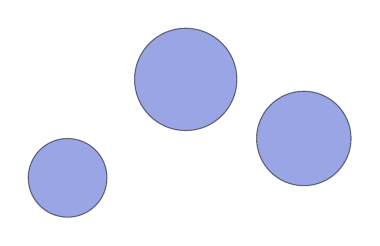
\begin{tikzpicture}[scale=0.5]
    \draw [fill=mblue, opacity=0.5] circle [radius = 1];
    \draw (3, 2.5) [fill=mblue, opacity=0.5] circle [radius = 1.3];
    \draw (6, 1) [fill=mblue, opacity=0.5] circle [radius = 1.2];
  \end{tikzpicture}
\end{center}
In the above space, we have three path components.

This isn't really a very useful definition, since most spaces we care about are path-connected, ie. only have one path component. However, this is a first step at associating \emph{something} to spaces. We can view this as a ``toy model'' for the more useful definitions we will later have.

One important property of this $\pi_0$ is that not only does it associate a set to each topological space, but also associates a function between the corresponding sets to each continuous map.
\begin{prop}
  For any map $f: X\to Y$, there is a well-defined function
  \[
    \pi_0(f): \pi_0(X) \to \pi_0(Y),
  \]
  defined by
  \[
    \pi_0(f)([x]) = [f(x)].
  \]
  Furthermore,
  \begin{enumerate}
    \item If $f\sim g$, then $\pi_0(f) = \pi_0(g)$.
    \item For any maps $\begin{tikzcd} A \ar[r, "h"] & B\ar[r, "k"] & C\end{tikzcd}$, we have $\pi_0(k\circ h) = \pi_0(k)\circ \pi_0 (h)$.
    \item $\pi_0(\id_X) = \id_{\pi_0(x)}$
  \end{enumerate}
\end{prop}
Proof is left as an easy exercise.

\begin{cor}
  If $f: X\to Y$ is a homotopy equivalence, then $\pi_0(f)$ is a bijection.
\end{cor}

\begin{eg}
  The two point space $X = \{-1, 1\}$ is not contractible. Because $|\pi_0(X)|$, but $|\pi_0(*)| = 1$.
\end{eg}
This is a rather silly example, since we can easily prove it directly. However, this is an example to show how we can use these machinery to prove topological results.

Now let's return to our operations on paths, and try to make them algebraic.

\begin{defi}[Homotopy of paths]
  Paths $\gamma, \gamma': I\to X$ are \emph{homotopic as paths} if they are homotopic rel $\{0, 1\}\subseteq I$, ie. the end points are fixed. We write $\gamma\simeq \gamma'$.
\end{defi}
\begin{center}
  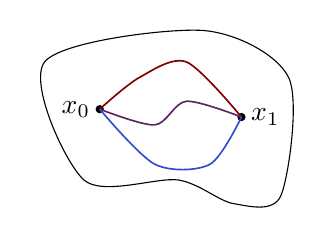
\begin{tikzpicture}
    \draw plot [smooth cycle] coordinates {(-1.2, -0.7) (0, -0.7) (0.7, -1) (1.3, -0.9) (1.4, 0.6) (0.3, 1.2) (-1.7, 0.8)};

    \node [circ] at (-1, 0.2) {};
    \node [left] at (-1, 0.2) {$x_0$};
    \node [circ] at (0.8, 0.1) {};
    \node [right] at (0.8, 0.1) {$x_1$};
    \draw [semithick, mred] plot [smooth] coordinates {(-1, 0.2) (-0.5, 0.6) (0.1, 0.8) (0.8, 0.1)};
    \draw [semithick, mred!50!mblue] plot [smooth] coordinates {(-1, 0.2) (-0.3, 0) (0.1, 0.3) (0.8, 0.1)};
    \draw [semithick, mblue] plot [smooth] coordinates {(-1, 0.2) (-0.3, -0.5) (0.4, -0.5) (0.8, 0.1)};
  \end{tikzpicture}
\end{center}
Note that we would necessarily want to fix the two end points. Otherwise, if we allow end points to move, we can shrink any path into a constant path, and our definition of homotopy would be rather silly.

This homotopy works well with our previous operations on paths.
\begin{prop}
  Let $\gamma_1, \gamma_2: I \to X$ be paths, $\gamma_1(1) = \gamma_2(0)$. Then if $\gamma_1\simeq \gamma_1'$ and $\gamma_2 \simeq \gamma_2'$, then $\gamma_1 \cdot \gamma_2 \simeq \gamma_1' \cdot \gamma_2'$.
\end{prop}
\begin{center}
  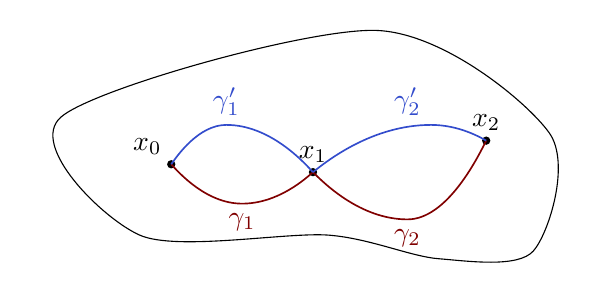
\begin{tikzpicture}
    \draw plot [smooth cycle] coordinates {(-2.4, -0.7) (0, -0.7) (1.4, -1) (2.6, -0.9) (2.8, 0.6) (0.6, 1.9) (-3.4, 0.8)};

    \node [circ] at (-2, 0.2) {};
    \node [anchor = south east] at (-2, 0.2) {$x_0$};
    \node [circ] at (-0.2, 0.1) {};
    \node [above] at (-0.2, 0.1) {$x_1$};
    \node [circ] at (2, 0.5) {};
    \node [above] at (2, 0.5) {$x_2$};
    \draw [semithick, mred] (-2, 0.2) parabola bend (-1.1, -0.3) (-0.2, 0.1);
    \draw [semithick, mred] (-0.2, 0.1) parabola bend (1, -0.5) (2, 0.5);

    \draw [semithick, mblue] (-2, 0.2) parabola bend (-1.3, 0.7) (-0.2, 0.1);
    \draw [semithick, mblue] (-0.2, 0.1) parabola bend (1.3, 0.7) (2, 0.5);

    \node [mred, below] at (-1.1, -0.3) {$\gamma_1$};
    \node [mred, below] at (1, -0.5) {$\gamma_2$};

    \node [mblue, above] at (-1.3, 0.7) {$\gamma_1'$};
    \node [mblue, above] at (1, 0.7) {$\gamma_2'$};
  \end{tikzpicture}
\end{center}

\begin{proof}
  Suppose that $\gamma_1 \simeq_{H_1}\gamma_1'$ and $\gamma_2\simeq_{H_2}\gamma_2'$. Then we have the diagram
  \begin{center}
    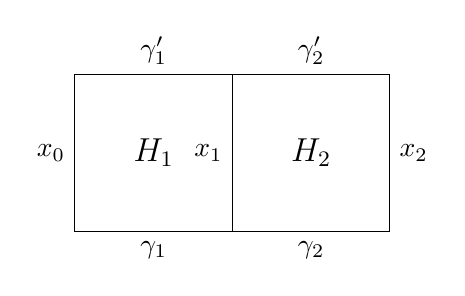
\begin{tikzpicture}
      \draw (0, 0) rectangle (2, 2);
      \draw (2, 0) rectangle (4, 2);
      \node at (1, 0) [below] {$\gamma_1$};
      \node at (3, 0) [below] {$\gamma_2$};
      \node at (1, 2) [above] {$\gamma_1'$};
      \node at (3, 2) [above] {$\gamma_2'$};
      \node at (0, 1) [left] {$x_0$};
      \node at (2, 1) [left] {$x_1$};
      \node at (4, 1) [right] {$x_2$};

      \node at (1, 1) {\large $H_1$};
      \node at (3, 1) {\large $H_2$};
    \end{tikzpicture}
  \end{center}
  We can thus construct a homotopy by
  \[
    H(s, t) =
    \begin{cases}
      H_1(s, 2t) & 0 \leq t \leq \frac{1}{2}\\
      H_2(s, 2t - 1) & \frac{1}{2} \leq t \leq 1
    \end{cases}.
  \]
\end{proof}

To solve all our previous problems about operations on paths not behaving well, we can look at paths \emph{up to homotopy}.
\begin{prop}
  Let $\gamma_0: x_0 \leadsto x_1, \gamma_1: x_1 \leadsto x_2, \gamma_2: x_2 \leadsto x_3$ be paths. Then
  \begin{enumerate}
    \item $(\gamma_0 \cdot \gamma_1)\cdot \gamma_2 \simeq \gamma_0 \cdot (\gamma_1\cdot \gamma_2)$
    \item $\gamma_0 \cdot c_{x_1}\simeq \gamma_0 \simeq c_{x_0}\cdot \gamma_0$.
    \item $\gamma_0 \cdot \gamma_0^{-1}\simeq c_{x_0}$ and $\gamma_0^{-1}\cdot \gamma_0 \simeq c_{x_1}$.
  \end{enumerate}
\end{prop}

\begin{proof}\leavevmode
  \begin{enumerate}
    \item Consider the following diagram:
      \begin{center}
        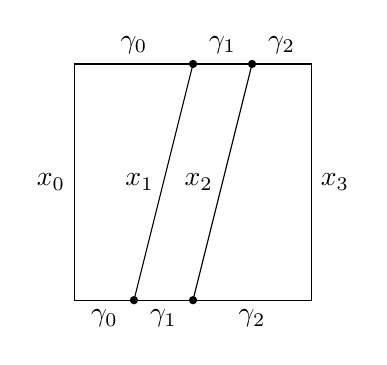
\begin{tikzpicture}[scale=0.75]
          \draw rectangle (4, 4);

          \node at (0, 2) [left] {$x_0$};
          \node at (4, 2) [right] {$x_3$};

          \node [circ] at (1, 0) {};
          \node [circ] at (2, 0) {};
          \node [circ] at (2, 4) {};
          \node [circ] at (3, 4) {};

          \node [below] at (0.5, 0) {$\gamma_0$};
          \node [below] at (1.5, 0) {$\gamma_1$};
          \node [below] at (3, 0) {$\gamma_2$};

          \node [above] at (1, 4) {$\gamma_0$};
          \node [above] at (2.5, 4) {$\gamma_1$};
          \node [above] at (3.5, 4) {$\gamma_2$};

          \draw (1, 0) -- (2, 4) node [pos=0.5, left] {$x_1$};
          \draw (2, 0) -- (3, 4) node [pos=0.5, left] {$x_2$};
        \end{tikzpicture}
      \end{center}
    \item Consider the following diagram:
      \begin{center}
        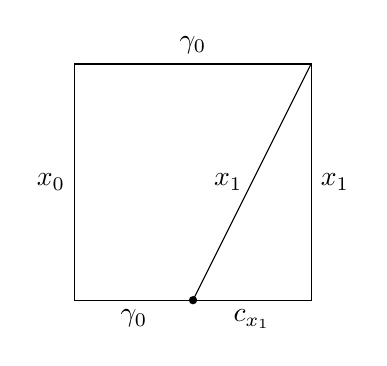
\begin{tikzpicture}[scale=0.75]
          \draw rectangle (4, 4);
          \node [circ] at (2, 0) {};
          \node at (1, 0) [below] {$\gamma_0$};
          \node at (3, 0) [below] {$c_{x_1}$};
          \node at (2, 4) [above] {$\gamma_0$};
          \node at (0, 2) [left] {$x_0$};
          \node at (4, 2) [right] {$x_1$};

          \draw (2, 0) -- (4, 4) node [pos=0.5, left] {$x_1$};
        \end{tikzpicture}
      \end{center}
    \item Consider the following diagram:
      \begin{center}
        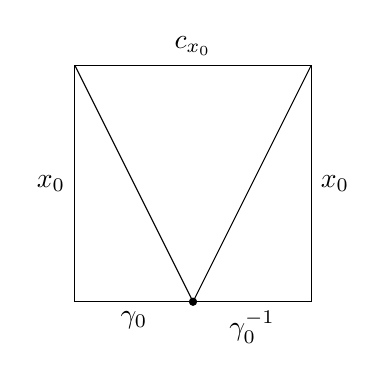
\begin{tikzpicture}[scale=0.75]
          \draw rectangle (4, 4);
          \node [circ] at (2, 0) {};
          \node at (1, 0) [below] {$\gamma_0$};
          \node at (3, 0) [below] {$\gamma_0^{-1}$};
          \node at (2, 4) [above] {$c_{x_0}$};
          \node at (0, 2) [left] {$x_0$};
          \node at (4, 2) [right] {$x_0$};

          \draw (0, 4) -- (2, 0) -- (4, 4);
        \end{tikzpicture}
      \end{center}
  \end{enumerate}
\end{proof}
\subsection{The fundamental group}
The idea is to take spaces and turn them into groups. We want to try to do this using paths. We've seen that if we want to do this, we should work directly with paths, but paths up to homotopy. According to our proposition, this operation satisfies associativity, inverses and identity. The last issue we have to resolve is that we can't actually put two paths together unless they have the same start and end points.

The idea is to fix one of the points $x_0$ in our space, and only think about loops that start and end at $x_0$. So we can always join two paths together.

This tells us that we aren't going to just think about spaces, but spaces \emph{with basepoints}. We've now got everything we need.

\begin{defi}[Fundamental group]
  Let $X$ be a space and $x_0 \in X$. The \emph{fundamental group} of $X$ (based at $x_0$), denoted $\pi_1(X, x_0)$, is the set of homotopy classes of loops in $X$ based at $x_0$ (ie. $\gamma(0) = \gamma(1) = x_0$). The group operations are defined as follows:

  We define an operation by $[\gamma_0][\gamma_1] = [\gamma_0\cdot \gamma_1]$; inverses by $[\gamma]^{-1} = [\gamma^{-1}]$; and the identity as the constant path $e = [c_{x_0}]$.
\end{defi}
Often, when we write the homotopy classes of paths $[\gamma]$, we just get lazy and write $\gamma$.

\begin{thm}[]
  The fundamental group is a group.
\end{thm}

\begin{proof}
  Immediate from our previous lemmas.
\end{proof}

Often, in mathematics, after defining a term, we give lots of examples of it. Unfortunately, it is rather difficult to prove that a space has a non-trivial fundamental group, until we have developed some relevant machinery. Hence we will have to wait for a while before we have some concrete examples. Instead, we will look at some properties of the fundamental group first.

\begin{defi}[Based space]
  A \emph{based space} is a pair $(X, x_0)$ of a space $X$ and a point $x_0\in X$, the \emph{basepoint}. A \emph{map of based spaces}
  \[
    f: (X, x_0) \to (Y, y_0)
  \]
  is a continuous map $f: X\to Y$ such that $f(x_0) = y_0$. A \emph{based homotopy} is a homotopy rel $\{x_0\}$.
\end{defi}

Recall that for $\pi_0$, for every map $f: X\to Y$, we can associate a function $\pi_0(f): \pi_0(X) \to \pi_0(Y)$. We can do the same for $\pi_1$.
\begin{prop}
  To a based map
  \[
    f: (X, x_0) \to (Y, y_0),
  \]
  there is an associated function
  \[
    f_* = \pi_1(f): \pi_1(X, x_0) \to \pi_1(Y, y_0),
  \]
  defined by $[\gamma] \mapsto [f\circ \gamma]$. Moreover, it satisfies
  \begin{enumerate}
    \item $\pi_1(f)$ is a homomorphism of groups.
    \item If $f \simeq f'$, then $\pi_1(f) = \pi_1(f')$.
    \item For any maps $\begin{tikzcd} (A, a) \ar[r, "h"] & (B, b) \ar[r, "k"] & (C, c) \end{tikzcd}$, we have $\pi_1(k\circ h) = \pi_1(k)\circ \pi_1 (h)$.
    \item $\pi_1(\id_X) = \id_{\pi_1(X, x_0)}$
  \end{enumerate}
\end{prop}

\begin{proof}
  Exercise.
\end{proof}
In category-theoretic language, we say that $\pi_1$ is a \emph{functor}.

So far so good. However, to define the fundamental group, we had to make a compromise and pick a basepoint. But we just care about the space. We don't want a basepoint! Hence, we should look carefully what happens when we change the basepoint, and see if we can live without it.

The first observation is that $\pi_1(X, x_0)$ only ``sees'' the path component of $x_0$, since all loops based at $x_0$ can only live inside the path component of $x_0$. Hence, the first importance of picking a basepoint is picking a path component.

For all practical purposes, we just assume that $X$ is path connected, since if we weren't, the fundamental group just describes a particular path component of the original space.

Now we want to compare fundamental groups with different basepoints. Suppose we have two basepoints $x_0$ and $x_1$. Suppose we have a loop $\gamma$ at $x_0$. How can we turn this into a loop based at $x_1$? This is easy. We first pick a path $u: x_0 \leadsto x_1$. Then we can produce a new loop at $x_1$ by going along $u^{-1}$ to $x_0$, take the path $\gamma$, and then return to $x_0$ by $u$, ie. consider $u\cdot \gamma\cdot u^{-1}$.
\begin{center}
  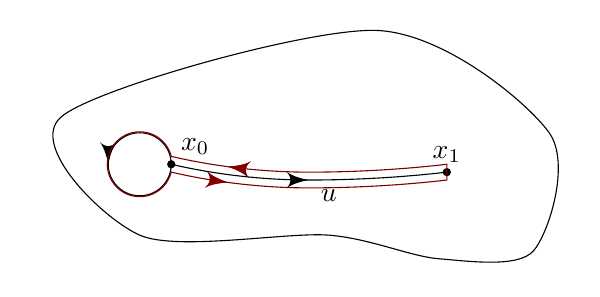
\begin{tikzpicture}
    \draw plot [smooth cycle] coordinates {(-2.4, -0.7) (0, -0.7) (1.4, -1) (2.6, -0.9) (2.8, 0.6) (0.6, 1.9) (-3.4, 0.8)};

    \node [circ] at (-2, 0.2) {};
    \node [anchor = south west] at (-2, 0.2) {$x_0$};
    \node [circ] at (1.5, 0.1) {};
    \node [above] at (1.5, 0.1) {$x_1$};

    \draw [->-=0.5] (-2.4, 0.2) circle [radius = 0.4];
    \draw [->-=0.5] (-2, 0.2) parabola bend (-0.25, 0) (1.5, 0.1) node [pos=0.5, below] {$u$};
    \draw [mred, ->-=0.3, ->-=0.7] (1.5, 0.1) -- (1.5, 0.2) parabola bend (-0.25, 0.1) (-2, 0.3) arc (14:346:0.4123) parabola bend (-0.25, -0.1) (1.5, 0) -- (1.5, 0.1);
  \end{tikzpicture}
\end{center}

\begin{prop}
  A path $u: x_0 \leadsto x_1$ induces a group \emph{isomorphism}
  \[
    u_\#: \pi_1(X, x_0) \to \pi_1(X, x_1)
  \]
  by
  \[
    [\gamma_0] \mapsto [u^{-1}\cdot \gamma \cdot u].
  \]
  This satisfies
  \begin{enumerate}
    \item If $u\simeq u'$, then $u_\# = u'_\#$.
    \item $(c_{x_0})_\# = \id_{\pi_1(X, x_0)}$
    \item If $v: x_1 \leadsto x_2$. Then $(u\cdot v)_\# = v_\# \circ u_\#$.
    \item If $f: X\to Y$ with $f(x_0) = y_0$, $f(x_1) = y_1$, then
      \[
        (f\circ u)_\# \circ f_* = f_* \circ u_\#: \pi_1(X, x_0) \to \pi_1(Y, y_1).
      \]
      A nicer way of writing this is
      \[
        \begin{tikzcd}[row sep=large]
          \pi_1(X, x_0) \ar[r, "f_*"] \ar[d, "u_\#"] & \pi_1(Y, y_0)\ar [d, "(f\circ u)_\#"]\\
          \pi_1(X, x_1) \ar[r, "f_*"] & \pi_1(Y, y_1)
        \end{tikzcd}
      \]
      The property says that the composition is the same no matter which way we go from $\pi_1(X, x_0)$ to $\pi_1(Y, y_1)$. We say that the square is a \emph{commutative diagram}. These diagrams will appear all of the time in this course.
    \item If $x_1 = x_0$, then $u_\#$ is an automorphism of $\pi_1(X, x_0)$ given by conjugation by $u$.
  \end{enumerate}
\end{prop}
It is important (yet difficult) the get the order of concatenation and composition right. Path concatenation is from left to right, while function composition is from right to left.

\begin{proof}
  Yet another exercise. Note that $(u^{-1})_\# = (u_\#)^{-1}$, which is why we have an isomorphism.
\end{proof}
The main takeaway is that if $x_0$ and $x_1$ are in the same path component, then 
\[
  \pi_1(X, x_0) \cong \pi_1(X, x_1).
\]
So the basepoint isn't really too important. However, we have to be careful. While the two groups are isomorphic, the actual isomorphism depends on \emph{which} path $u: x_0 \leadsto x_1$ we pick. So there is no natural isomorphism between the two groups. In particular, we cannot say ``let $\alpha \in \pi_1(X, x_0)$. Now let $\alpha'$ be the corresponding element in $\pi_1(X, x_1)$''.

We can also see if $(X, x_0)$ and $(Y, y_0)$ are based homotopy equivalent, then $\pi_1(X, x_0)\cong \pi_1(Y, y_0)$. Indeed, if they are homotopy equivalent, then there is some $f: X \to Y$, $g: Y \to X$ such that $f\circ g = \id_Y$, $g\circ f = \id_X$. So $f_*\circ g_* = \id_{\pi_1(Y, y_0)}$ and $g_*\circ f_* = \id_{\pi_1(X, x_0)}$, and $f_*$ and $g_*$ are the isomorphisms we need.

However, can we do this with non-based homotopies? Suppose we have a space $X$, and a space $Y$, and functions $f, g: X \to Y$, with a homotopy $H: X\times I \to Y$ from $f$ to $g$. Since we don't insist that this fixes $x_0$, we could have $f(x_0) \not= g(x_0)$. What can we do?

First of all, we can find a path from $f(x_0)$ to $g(x_0)$. To produce this, we can use the homotopy. We let $u: f(x_0) \leadsto g(x_0)$ with $u = H(x_0, \cdot)$. Now we have things like $f_*, g_*$ and $u_\#$. Fortunately, these do fit together well.
\begin{center}
  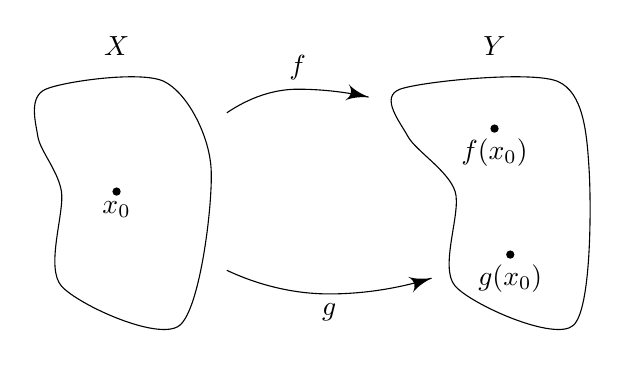
\begin{tikzpicture}
    \draw plot [smooth cycle] coordinates {(-3.7, -1.2) (-3.7, 0) (-4, 0.7) (-3.9, 1.3) (-2.4, 1.4) (-1.8, 0.3) (-2.2, -1.7)};
    \draw plot [smooth cycle] coordinates {(1.3, -1.2) (1.3, 0) (0.7, 0.7) (0.6, 1.3) (2.6, 1.4) (3, 0.3) (2.8, -1.7)};

    \node [circ] at (-3, 0) {};
    \node [below] at (-3, 0) {$x_0$};
    \node [above] at (-3, 1.6) {$X$};

    \node [above] at (1.8, 1.6) {$Y$};

    \node [circ] at (1.8, 0.8) {};
    \node [below] at (1.8, 0.8) {$f(x_0)$};

    \node [circ] at (2, -0.8) {};
    \node [below] at (2, -0.8) {$g(x_0)$};

    \draw [->] (-1.6, 1) parabola bend (-0.7, 1.3) (0.2, 1.2);
    \node [above] at (-0.7, 1.3) {$f$};

    \draw [->] (-1.6, -1) parabola bend (-0.3, -1.3) (1, -1.1);
    \node [below] at (-0.3, -1.3) {$g$};
  \end{tikzpicture}
\end{center}

\begin{lemma}
  The following diagram commutes:
  \[
    \begin{tikzcd}
      & \pi_1(Y, f(x_0)) \ar[dd, "u_\#"]\\
      \pi_1(X, x_0) \ar[ru, "f_*"] \ar [rd, "g_*"']& \\
      & \pi_1(Y, g(x_0))
    \end{tikzcd}
  \]
  In algebra, we say
  \[
    g_* = u_\# \circ f_*.
  \]
\end{lemma}
\end{document}
